% Options for packages loaded elsewhere
\PassOptionsToPackage{unicode}{hyperref}
\PassOptionsToPackage{hyphens}{url}
\PassOptionsToPackage{dvipsnames,svgnames,x11names}{xcolor}
%
\documentclass[
]{article}

\usepackage{amsmath,amssymb}
\usepackage{iftex}
\ifPDFTeX
  \usepackage[T1]{fontenc}
  \usepackage[utf8]{inputenc}
  \usepackage{textcomp} % provide euro and other symbols
\else % if luatex or xetex
  \usepackage{unicode-math}
  \defaultfontfeatures{Scale=MatchLowercase}
  \defaultfontfeatures[\rmfamily]{Ligatures=TeX,Scale=1}
\fi
\usepackage{lmodern}
\ifPDFTeX\else  
    % xetex/luatex font selection
\fi
% Use upquote if available, for straight quotes in verbatim environments
\IfFileExists{upquote.sty}{\usepackage{upquote}}{}
\IfFileExists{microtype.sty}{% use microtype if available
  \usepackage[]{microtype}
  \UseMicrotypeSet[protrusion]{basicmath} % disable protrusion for tt fonts
}{}
\makeatletter
\@ifundefined{KOMAClassName}{% if non-KOMA class
  \IfFileExists{parskip.sty}{%
    \usepackage{parskip}
  }{% else
    \setlength{\parindent}{0pt}
    \setlength{\parskip}{6pt plus 2pt minus 1pt}}
}{% if KOMA class
  \KOMAoptions{parskip=half}}
\makeatother
\usepackage{xcolor}
\usepackage[margin=1in]{geometry}
\setlength{\emergencystretch}{3em} % prevent overfull lines
\setcounter{secnumdepth}{5}
% Make \paragraph and \subparagraph free-standing
\makeatletter
\ifx\paragraph\undefined\else
  \let\oldparagraph\paragraph
  \renewcommand{\paragraph}{
    \@ifstar
      \xxxParagraphStar
      \xxxParagraphNoStar
  }
  \newcommand{\xxxParagraphStar}[1]{\oldparagraph*{#1}\mbox{}}
  \newcommand{\xxxParagraphNoStar}[1]{\oldparagraph{#1}\mbox{}}
\fi
\ifx\subparagraph\undefined\else
  \let\oldsubparagraph\subparagraph
  \renewcommand{\subparagraph}{
    \@ifstar
      \xxxSubParagraphStar
      \xxxSubParagraphNoStar
  }
  \newcommand{\xxxSubParagraphStar}[1]{\oldsubparagraph*{#1}\mbox{}}
  \newcommand{\xxxSubParagraphNoStar}[1]{\oldsubparagraph{#1}\mbox{}}
\fi
\makeatother


\providecommand{\tightlist}{%
  \setlength{\itemsep}{0pt}\setlength{\parskip}{0pt}}\usepackage{longtable,booktabs,array}
\usepackage{calc} % for calculating minipage widths
% Correct order of tables after \paragraph or \subparagraph
\usepackage{etoolbox}
\makeatletter
\patchcmd\longtable{\par}{\if@noskipsec\mbox{}\fi\par}{}{}
\makeatother
% Allow footnotes in longtable head/foot
\IfFileExists{footnotehyper.sty}{\usepackage{footnotehyper}}{\usepackage{footnote}}
\makesavenoteenv{longtable}
\usepackage{graphicx}
\makeatletter
\def\maxwidth{\ifdim\Gin@nat@width>\linewidth\linewidth\else\Gin@nat@width\fi}
\def\maxheight{\ifdim\Gin@nat@height>\textheight\textheight\else\Gin@nat@height\fi}
\makeatother
% Scale images if necessary, so that they will not overflow the page
% margins by default, and it is still possible to overwrite the defaults
% using explicit options in \includegraphics[width, height, ...]{}
\setkeys{Gin}{width=\maxwidth,height=\maxheight,keepaspectratio}
% Set default figure placement to htbp
\makeatletter
\def\fps@figure{htbp}
\makeatother

\makeatletter
\@ifpackageloaded{caption}{}{\usepackage{caption}}
\AtBeginDocument{%
\ifdefined\contentsname
  \renewcommand*\contentsname{Table of contents}
\else
  \newcommand\contentsname{Table of contents}
\fi
\ifdefined\listfigurename
  \renewcommand*\listfigurename{List of Figures}
\else
  \newcommand\listfigurename{List of Figures}
\fi
\ifdefined\listtablename
  \renewcommand*\listtablename{List of Tables}
\else
  \newcommand\listtablename{List of Tables}
\fi
\ifdefined\figurename
  \renewcommand*\figurename{Figure}
\else
  \newcommand\figurename{Figure}
\fi
\ifdefined\tablename
  \renewcommand*\tablename{Table}
\else
  \newcommand\tablename{Table}
\fi
}
\@ifpackageloaded{float}{}{\usepackage{float}}
\floatstyle{ruled}
\@ifundefined{c@chapter}{\newfloat{codelisting}{h}{lop}}{\newfloat{codelisting}{h}{lop}[chapter]}
\floatname{codelisting}{Listing}
\newcommand*\listoflistings{\listof{codelisting}{List of Listings}}
\makeatother
\makeatletter
\makeatother
\makeatletter
\@ifpackageloaded{caption}{}{\usepackage{caption}}
\@ifpackageloaded{subcaption}{}{\usepackage{subcaption}}
\makeatother

\ifLuaTeX
  \usepackage{selnolig}  % disable illegal ligatures
\fi
\usepackage{bookmark}

\IfFileExists{xurl.sty}{\usepackage{xurl}}{} % add URL line breaks if available
\urlstyle{same} % disable monospaced font for URLs
\hypersetup{
  pdftitle={Pontificia Universidad Javeriana},
  pdfauthor={Matemáticas Para Biologia I},
  colorlinks=true,
  linkcolor={blue},
  filecolor={Maroon},
  citecolor={Blue},
  urlcolor={Blue},
  pdfcreator={LaTeX via pandoc}}


\title{Pontificia Universidad Javeriana}
\author{Matemáticas Para Biologia I}
\date{}

\begin{document}
\maketitle


\section{Taller de máximos y
mínimos}\label{taller-de-muxe1ximos-y-muxednimos}

\begin{enumerate}
\def\labelenumi{\arabic{enumi}.}
\item
  Encuentra dos números cuya diferencia es 100 y cuyo producto es
  mínimo.
\item
  Encuentra dos números positivos cuyo producto es 100 y cuya suma es
  mínima.
\item
  La suma de dos números positivos es 16. ¿Cuál es el valor mínimo
  posible de la suma de sus cuadrados?
\item
  Encuentra las dimensiones de un rectángulo con un perímetro de 100
  metros cuyo área es la mayor posible.
\item
  Observe las siguientes gráficas de funciones polinomiales, haga el
  bosquejo de la primera y segunda derivada de cada una de ellas y
  determine los puntos críticos de cada función, máximos, mínimos y
  puntos de inflexión.
\end{enumerate}

\begin{verbatim}
No artists with labels found to put in legend.  Note that artists whose label start with an underscore are ignored when legend() is called with no argument.
\end{verbatim}

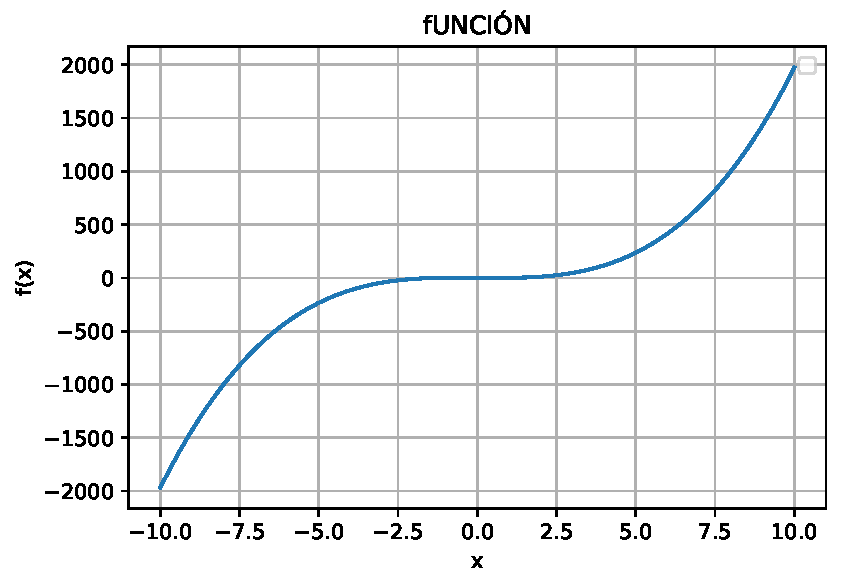
\includegraphics{taller_maximos_files/figure-pdf/cell-2-output-2.pdf}

\begin{enumerate}
\def\labelenumi{\arabic{enumi}.}
\setcounter{enumi}{5}
\tightlist
\item
  \textbf{Problema: Forrajeo de néctar por abejorros}
\end{enumerate}

Muchos animales forrajean recursos que están distribuidos en parches
discretos. Por ejemplo, los abejorros visitan muchas flores,
recolectando néctar de cada una. La cantidad de néctar \(N(t)\)
consumida de cualquier flor aumenta con el tiempo que el abejorro pasa
en esa flor, pero con rendimientos decrecientes. Supongamos que esta
función está dada por:

\[
N(t) = \frac{0.3t}{t+2}
\]

donde \(t\) se mide en segundos y \(N(t)\) en miligramos. Supongamos
también que el tiempo que tarda una abeja en viajar de una flor a la
siguiente es de 4 segundos.

\begin{enumerate}
\def\labelenumi{\alph{enumi}.}
\item
  Si una abeja pasa \(t\) segundos en cada flor, encuentra una ecuación
  para la cantidad promedio de néctar consumido por segundo, desde el
  comienzo de la visita a una flor hasta el comienzo de la visita a la
  siguiente flor.
\item
  Supongamos que los abejorros forrajean en una flor por un tiempo que
  maximiza la tasa promedio de consumo de néctar obtenida en la parte
  (a). ¿Cuál es este tiempo de forrajeo óptimo?
\end{enumerate}

\begin{enumerate}
\def\labelenumi{\arabic{enumi}.}
\setcounter{enumi}{6}
\item
  \textbf{Lanzamiento} Un hombre lanza su bote desde el punto A en la
  orilla de un canal de agua recto, que tiene 3 km de ancho, y quiere
  llegar al punto B, ubicado 8 km al sur en la orilla opuesta, lo más
  rápido posible (ver Figura 5). Podría remar su bote directamente a
  través del canal hasta el punto C y luego correr hasta B, o podría
  remar directamente hasta B, o podría remar hasta algún punto D entre C
  y B y luego correr hasta B. Si puede remar a una velocidad de 6 km/h y
  correr a una velocidad de 8 km/h, ¿en qué punto debería desembarcar
  para llegar a B lo antes posible? (Suponemos que el agua en el canal
  no está en movimiento).
\item
  \textbf{Forrajeo de Aves Acuáticas}
\end{enumerate}

Las aves acuáticas forrajean bajo el agua y periódicamente regresan a la
superficie para reponer sus reservas de oxígeno. Las reservas de oxígeno
aumentan con la cantidad de tiempo que pasan en la superficie, pero de
manera decreciente, de acuerdo con el modelo:

\[
O(t) = \frac{20t}{5 + t}
\]

donde \(t\) es el tiempo que pasan en la superficie (en segundos).
Supongamos que el tiempo de viaje de ida y vuelta hacia y desde el área
de forrajeo bajo el agua es \(T\) segundos y que el oxígeno se consume a
una tasa constante de (r) mL/s mientras el ave está bajo el agua.
Además, supongamos que el ave forrajea hasta que tiene justo suficiente
oxígeno para regresar a la superficie.

\begin{enumerate}
\def\labelenumi{\alph{enumi}.}
\item
  Si (Q) es la fracción de un ciclo de buceo completo que el ave pasa
  forrajeando, encuentra una ecuación para (Q) como una función del
  tiempo en la superficie (t).
\item
  Si (T = 2) segundos y (r = 1) mL/s, encuentra el tiempo en la
  superficie (t) que maximiza la fracción de tiempo que pasa
  forrajeando.
\end{enumerate}

\begin{enumerate}
\def\labelenumi{\arabic{enumi}.}
\setcounter{enumi}{8}
\tightlist
\item
  \textbf{Pesca sostenible}
\end{enumerate}

Para muchas poblaciones naturales de peces, el número neto de nuevos
reclutas a la población en un año dado puede modelarse como una función
del tamaño de la población existente (N), mediante una ecuación de la
forma:

\[
R(N) = rN\left(1 - \frac{N}{K}\right)
\]

donde (r) y (K) son constantes positivas. (A (K) se le llama la
capacidad de carga). La población aumentará si el número neto de
reclutas (R(N)) es positivo, y disminuirá si (R(N)) es negativo. Por lo
tanto, dado que (R(N)) es positivo cuando (0 \textless{} N \textless{}
K) y (R(N)) es negativo cuando (N \textgreater{} K), esperamos que la
población se estabilice en un tamaño constante de (N = K).

Si la población está sujeta a cosecha, (N) comenzará a cambiar y, una
vez que la población se haya estabilizado nuevamente, el número de peces
cosechados cada año, que denotamos por (H), debe ser igual al
reclutamiento neto de ese año; es decir:

\[
R(N) = H
\]

\begin{enumerate}
\def\labelenumi{\alph{enumi}.}
\item
  Supongamos que (H = hN), donde (h) es una medida del ``esfuerzo de
  pesca'' realizado. ¿Cuál es el tamaño de la población una vez que se
  ha estabilizado?
\item
  Expresa la tasa total de cosecha (H) como una función de (h) una vez
  que la población se haya estabilizado, y determina el esfuerzo de
  pesca que resulta en la mayor tasa de cosecha posible.
\item
  ¿Cuál es el tamaño de la población una vez que se ha estabilizado si
  se utiliza este esfuerzo de pesca óptimo, y cuál es la cosecha total?
\end{enumerate}

\begin{enumerate}
\def\labelenumi{\arabic{enumi}.}
\setcounter{enumi}{9}
\tightlist
\item
  \textbf{Saranpio} La función de patogénesis del sarampión:
\end{enumerate}

\[
f(t) = -t(t - 21)(t + 1)
\]

se utiliza en la Sección 5.1 para modelar el desarrollo de la
enfermedad, donde (t) se mide en días y (f(t)) representa el número de
células infectadas por mililitro de plasma. ¿Cuál es el tiempo de
infección máxima para el virus del sarampión?

\begin{enumerate}
\def\labelenumi{\arabic{enumi}.}
\setcounter{enumi}{10}
\tightlist
\item
  Un agricultor tiene 750 pies de cercado y quiere cercar un área
  rectangular, dividiéndola en cuatro corrales con cercado paralelo a un
  lado del rectángulo. ¿Cuál es el área total más grande posible de los
  cuatro corrales?
\end{enumerate}

\begin{enumerate}
\def\labelenumi{\alph{enumi}.}
\item
  Dibuja varios diagramas que ilustren la situación, algunos con
  corrales anchos y poco profundos y otros con corrales profundos y
  estrechos. Calcula las áreas totales de estas configuraciones. ¿Parece
  que existe un área máxima? Si es así, estímala.
\item
  Dibuja un diagrama que ilustre la situación general. Introduce
  notación y etiqueta el diagrama con tus símbolos.
\item
  Escribe una expresión para el área total.
\item
  Usa la información proporcionada para escribir una ecuación que
  relacione las variables.
\end{enumerate}

\begin{enumerate}
\def\labelenumi{\arabic{enumi}.}
\setcounter{enumi}{11}
\tightlist
\item
  \textbf{Forrajeo de abejas 2}
\end{enumerate}

Supongamos que, en lugar de la función específica de néctar del
Ejercicio 6, tenemos una función arbitraria (N(t)) con las condiciones
(N(0) = 0), (N(t) \textgreater{} 0), (N'(t) \textgreater{} 0), (N'\,'(t)
\textless{} 0), y un tiempo de viaje arbitrario (T).

\begin{enumerate}
\def\labelenumi{\alph{enumi}.}
\item
  Interpreta las condiciones sobre la función (N(t)).
\item
  Demuestra que el tiempo de forrajeo óptimo (t) satisface la ecuación:
\end{enumerate}

\[
N'(t) = \frac{N(t)}{t + T}
\]

\begin{enumerate}
\def\labelenumi{\alph{enumi}.}
\setcounter{enumi}{2}
\tightlist
\item
  Demuestra que, para cualquier tiempo de forrajeo (t) que satisfaga la
  ecuación en la parte (b), se cumple la condición de la segunda
  derivada para un valor máximo de la función de forrajeo (f) en el
  Ejercicio 6.
\end{enumerate}




\end{document}
